\subsection{The First Refinement}
\label{sec:component_diagrams-tutorial_firstRefinement}


The single component and abstract state machine is now refined into a system comprising two components as shown in Figure \ref{fig:FirstRefinementOfWashingMachine} below. The first component is the Control Panel and the second the abstract washing machine sub-system. Two connectors enable communication between the two components. The first connector, CI, is used to pass the Washing Program ID (PID) to the washing machine sub-system and the second connector, WMSTATE, passes the status of the sub-system back to the Control Panel to be displayed. The state machine is unchanged except for the addition of a self transition on state IDLE which constrains the sendWaiting operation so that it only sends the waiting status over the WMSTATE connector while the washing machine is idle.
 
 \begin{figure}[!htbp]
  \centering
  \ifplastex
  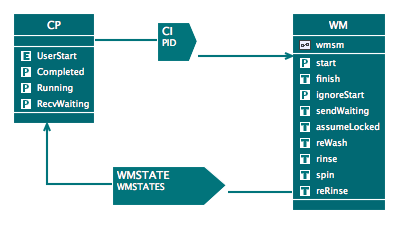
\includegraphics[width=1024]{figures/image19.png}
  \else
  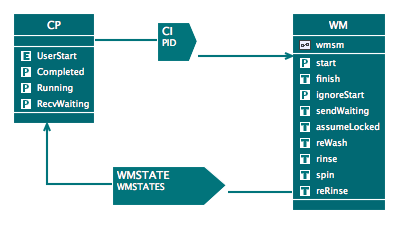
\includegraphics[width=1\textwidth]{figures/image19.png}
  \fi
  \caption{First Refinement of Washing Machine}
  \label{fig:FirstRefinementOfWashingMachine}
\end{figure} 

The external operation, UserStart, in component CP represents the user starting the wash by passing the selected wash program, using a port-send action on connector CI to the washing machine sub-system. The port-send action is shown in Figure \ref{fig: FirstRefinementPortSendsOnCI}. Note that the minimum delay of 1 is used. The value pid1 is a parameter representing the non-deterministic sending of any PID.
 
 \begin{figure}[!htbp]
  \centering
  \ifplastex
  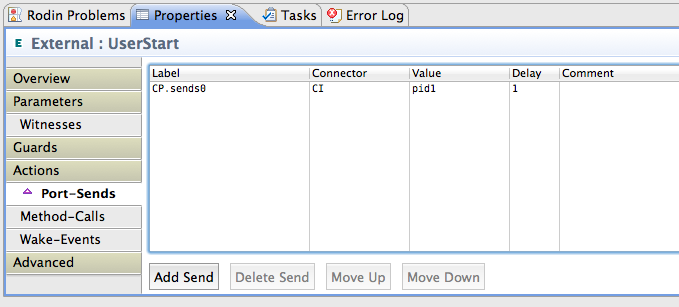
\includegraphics[width=1024]{figures/image20.png}
  \else
  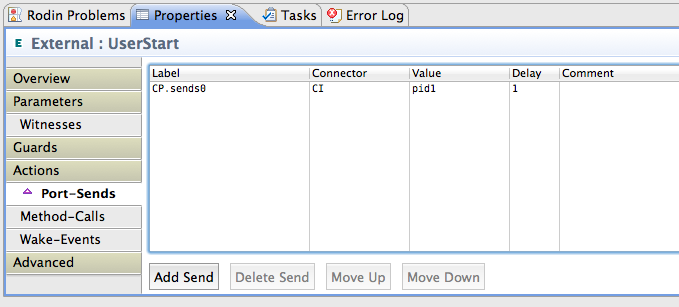
\includegraphics[width=1\textwidth]{figures/image20.png}
  \fi
  \caption{First Refinement : Port Sends on CI}
  \label{fig: FirstRefinementPortSendsOnCI}
\end{figure} 

A corresponding port-wake operation, start, in the washing machine sub-system receives the program ID that will, in a subsequent refinement, be decoded to control the wash. The port-wake guard is shown in Figure \ref{fig:FirstRefinementPortWakesOnCI}. 
A further port-wake operation, ignoreStart, manages inadvertent start requests from the user. Note that this is necessary due to a design decision not to constrain the sending of start messages from CP. If WM is not in a state to respond to the start an explicit ignoreStart is needed to avoid the system deadlocking.
 
 \begin{figure}[!htbp]
  \centering
  \ifplastex
  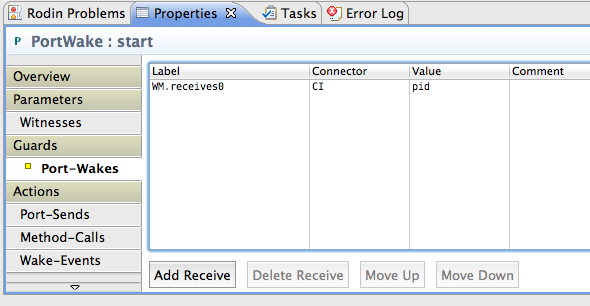
\includegraphics[width=1024]{figures/image21.png}
  \else
  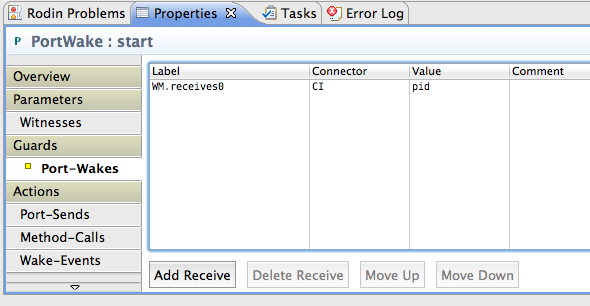
\includegraphics[width=1\textwidth]{figures/image21.png}
  \fi
  \caption{First Refinement : Port Wakes on CI}
  \label{fig:FirstRefinementPortWakesOnCI}
\end{figure} 

When the washing machine sub-system receives the pid, it responds with a port-send action on connector WMSTATE to inform the Control Panel that the washing machine is now RUNNING as shown in Figure \ref{fig:FirstRefinementPortSendsOnWMSTATE}.
 
 \begin{figure}[!htbp]
  \centering
  \ifplastex
  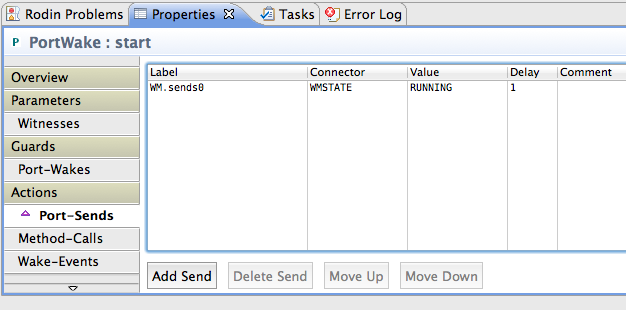
\includegraphics[width=1024]{figures/image22.png}
  \else
  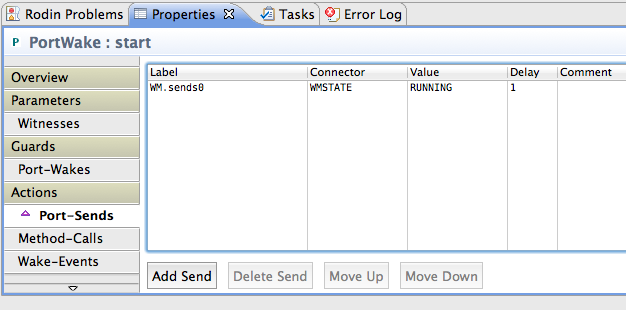
\includegraphics[width=1\textwidth]{figures/image22.png}
  \fi
  \caption{First Refinement : Port Sends on WMSTATE}
  \label{fig:FirstRefinementPortSendsOnWMSTATE}
\end{figure} 

The Control Panel receives the message from the washing machine sub-system with the port-wake operation Running shown in Figure \ref{fig:FirstRefinementPortWakesOnWMSTATE} so that this information can be displayed to the washing machine user.
 
 \begin{figure}[!htbp]
  \centering
  \ifplastex
  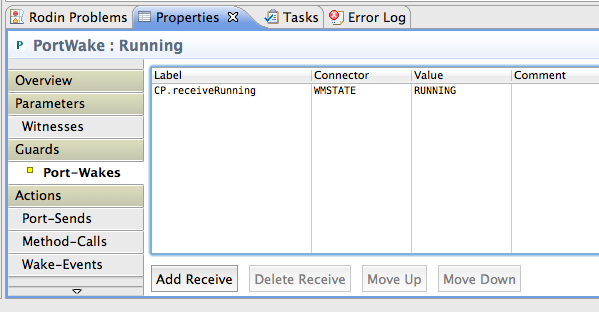
\includegraphics[width=1024]{figures/image23.png}
  \else
  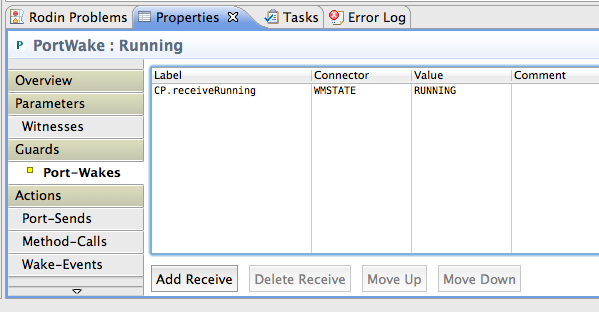
\includegraphics[width=1\textwidth]{figures/image23.png}
  \fi
  \caption{First Refinement : Port Wakes on WMSTATE}
  \label{fig:FirstRefinementPortWakesOnWMSTATE}
\end{figure} 

The State Machine Animation facility is now used again to validate this two component system and the model checker is run to check for deadlocks as shown in Figure \ref{fig:ProBModelCheckingCoverageForTheFirstRefinement}. Note that, again, all operations have been covered by the model checker.
 
 \begin{figure}[!htbp]
  \centering
  \ifplastex
  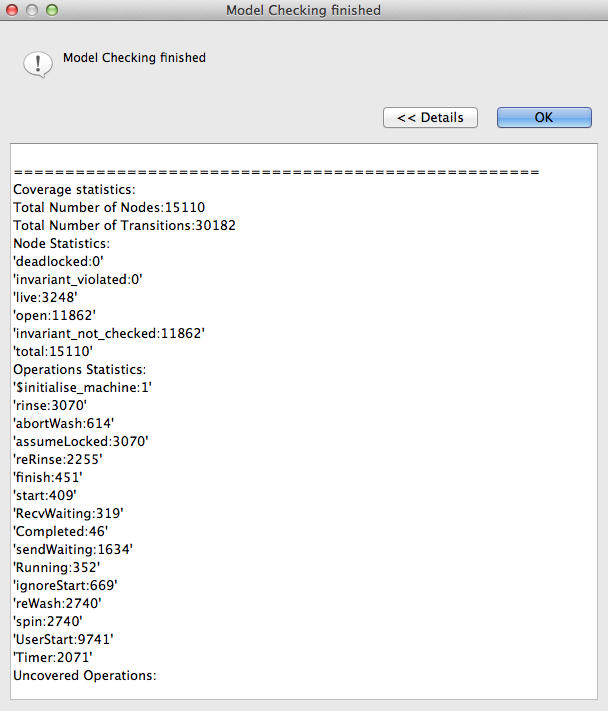
\includegraphics[width=1024]{figures/image24.png}
  \else
  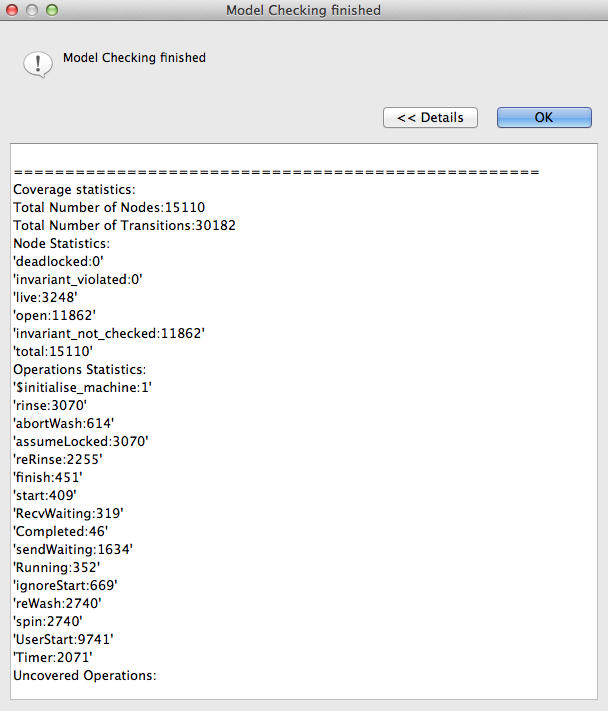
\includegraphics[width=1\textwidth]{figures/image24.png}
  \fi
  \caption{ProB Model Checking Coverage for the First Refinement}
  \label{fig:ProBModelCheckingCoverageForTheFirstRefinement}
\end{figure} 


%%% Local Variables:
%%% mode: latex
%%% TeX-master: "component_diagrams-user_manual"
%%% End:
